\chapter{Result and Discussion}
\label{Result and Discussion}
\section{Experimental scenarios}
Our evaluation is performed on a MacBook Pro as the Face recognition system; Raspberry Pi version 4 as the \acrlong{ccu} to control IoT devices. Table~\ref{tab:serverSpecs} summarizes the hardware configuration. The \acrlong{ccu} hardware configuration is mentioned in table~\ref{tab:raspiSpecsr}.

\begin{table}[H]
    \centering
    \caption{Face recognition server configuration}
    ~\\
    \begin{tabular}{|c|c|}
        \hline
        OS & macOS Mojave 10.14 \\
        \hline
        CPU & Intel(R) Core(TM) i7-3720QM \\
        \hline
        RAM & 16GB\\
        \hline
        GPU & NVIDIA GeForce GT 650M (1GB VRAM)\\
        \hline
    \end{tabular}
    \label{tab:serverSpecs}
\end{table}

\begin{table}[H]
    \centering
    \caption{\acrlong{ccu} specification}
    \begin{tabular}{|c|c|}
        \hline
        OS & Raspberry Pi OS (Linux based) \\
        \hline
        Kernel version & 5.10\\
        \hline
        CPU & Quad-core Cortex-A72 (ARM v8) 64-bit Soc \\
        \hline
        RAM & 4GB\\
        \hline
    \end{tabular}
    \label{tab:raspiSpecsr}
\end{table}

As face recognizing is memory intensive, Raspberry Pi can not compute as fast as on a server. So that to have a better user experience, we are choosing to implement the model on a MacBook Pro for testing. On a retail product, we may have to build up a server for each client.

Figure \ref{fig:prodSetup} shows the device setup diagram for evaluating, testing, and also in the public product:

\begin{figure}[H]
    \centering
    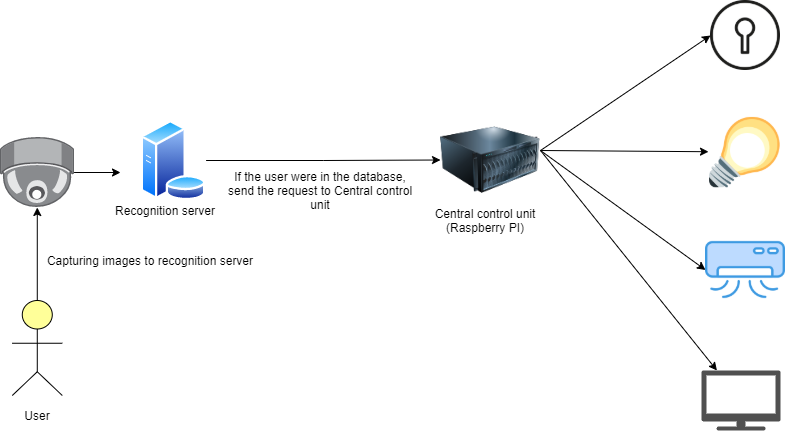
\includegraphics[scale=0.6]{setupDiag.png}
    \caption{Product flow}
    \label{fig:prodSetup}
\end{figure}

\section{System evaluation}
\subsection{Recognition system}
We are evaluating the model as the performance of the recognition system. The Confusion matrix is built to evaluate how well the model is.

\begin{table}[H]
    \centering
    \caption{Confusion matrix}
    \begin{tabular}{|c|c|c|}
        \hline
         &  Actual Negative &  Actual Positive\\
        \hline
        Predict Negative & True Negatives (TN) & False Negatives (FN)\\
        \hline
        Predict Positive & False Positive (FP) & True Positive (TP)\\
        \hline
    \end{tabular}
    \label{tab:confusionMatrix}
\end{table}
\begin{itemize}
    \item \textbf{Accuracy}: Accuracy is the value that shows how accurate  the model is, overall the class.
    \[
        Accuracy = \frac{TN+TP}{TN+FN+TP+FP}
    \]
    \item \textbf{Precision}: Precision defines how good the model is when predicting a class if the precision is low, meaning your model makes many mistakes in predicting.
    \[
        Precision = \frac{TP}{TP+FP}
    \]
    \item \textbf{Recall}: Recall(or Sensitivity) shows the accuracy of your model on the positive case, so the higher Recall, the better your model.
    \[
        Recall = \frac{TP}{TP+FN}
    \]
    \item \textbf{F1 score}: F1 score show the balance between Precision and Recall
    \[
        F1 = 2\times\frac{Precision*Recall}{Precision+Recall}
    \]
\end{itemize}

\begin{table}[H]
    \centering
    \caption{Evaluation with confusion matrix}
    \begin{tabular}{|c|c|c|c|c|}
        \hline
        Accuracy & Precision & Recall & F1 score \\
        \hline
        0.983740 & 0.986542 & 0.982919 & 0.983147 \\
        \hline
    \end{tabular}
\end{table}

We test the effective of the model by using a set of test images that includes many classes. Then the model will extract the embedding vectors for each image. After getting vectors, we use t-sine for reducing the dimensional of the vectors then visualize it.

\begin{figure}[H]
    \centering
    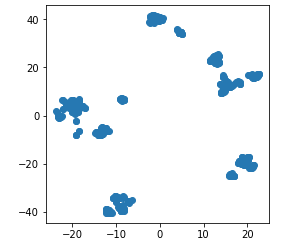
\includegraphics[scale=0.9]{tsneVisual.png}
    \caption{Scatter plot of the embedding vectors}
\end{figure}

For a better visual, we will show it on TensorBoard. The model works flawlessly on moving the picture of a same person together.

\begin{figure}[H]
    \centering
    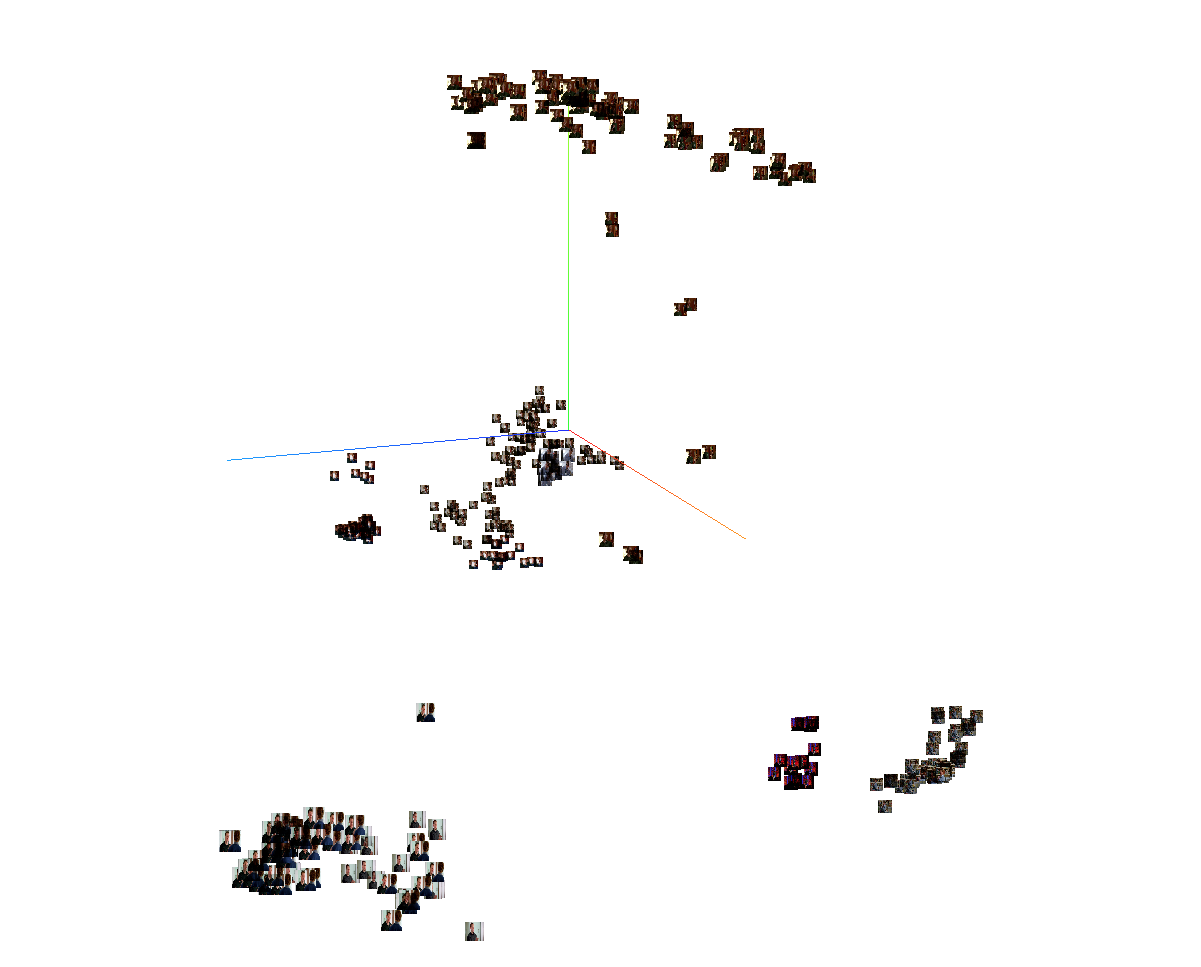
\includegraphics[scale=0.4]{tensorBoard.png}
    \caption{TensorBoard visualisation of embedding vectors}
\end{figure}

We applied the system onto our home on real-time usage, and it has an estimated 95\% accuracy based on successful unlock, failed to unlock.

Table~\ref{tab:trainingTime} shows the time of processing for each scenario (we choose one picture for each class):
\begin{table}[H]
    \centering
    \caption{Processing time for each scenario}
    \begin{tabular}{|c|c|}
        \hline
        Number of the registered person & Processing time(seconds) \\
        \hline
        3 & 2.17\\
        \hline
        100 & 39.18\\
        \hline
        4000 & 313\\
        \hline
    \end{tabular}
    \label{tab:trainingTime}
\end{table}

The processing time above indicates the time of calculating pictures to 128 dimension vectors. It can improve by using better hardware for less executing time.

\subsection{\acrlong{ccu} and \acrshort{api} performance}
\paragraph{}
The performance of \acrshort{ccu} is calculated on the percentage of success time and failed time. For most of the testing time, the system runs perfectly with a 100\% success rate.

About the \acrshort{api} connection, the only network connection can affect its performance. Since we shared a local network on both devices, \acrshort{api} runs without any delay.

\section{Discussion}
In everyday usage, our system works without any problems. But compare with other products on the market, there are some drawbacks to our approach:
\subsubsection{Inaccuracy with an extensive database}
\paragraph{}
On our evaluation, with an extensive database (more than 4000 people), the model seems not to recognize as accurately as before. Many elements can affect the performance, but we think that in a sizeable registered person, there will be a small percentage that two people can have a similar face landmarks as well as similar Euclidean vectors. That leads to an equal distance when compare them to each other.

We think that our model is not trained enough to extract more precise face landmarks. This problem can be solved by a well-trained model with a large dataset.

\subsubsection{Set up the system on multiple devices}
\paragraph{}
Many public products by large company that integrated all elements on only one device like in ~\ref{fig:publishedProd}. Compare with our product in ~\ref{fig:ccuSetup}, we have to implement it on two devices: one for recognition and one for control the lock, as well as other smart home devices.

\begin{figure}[H]
    \centering
    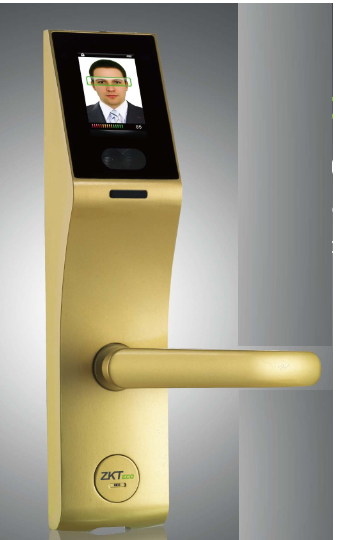
\includegraphics[scale=0.6]{marketProduct.png}
    \caption{An example of an on-sale product}
    \label{fig:publishedProd}
\end{figure}

\begin{figure}
    \centering
    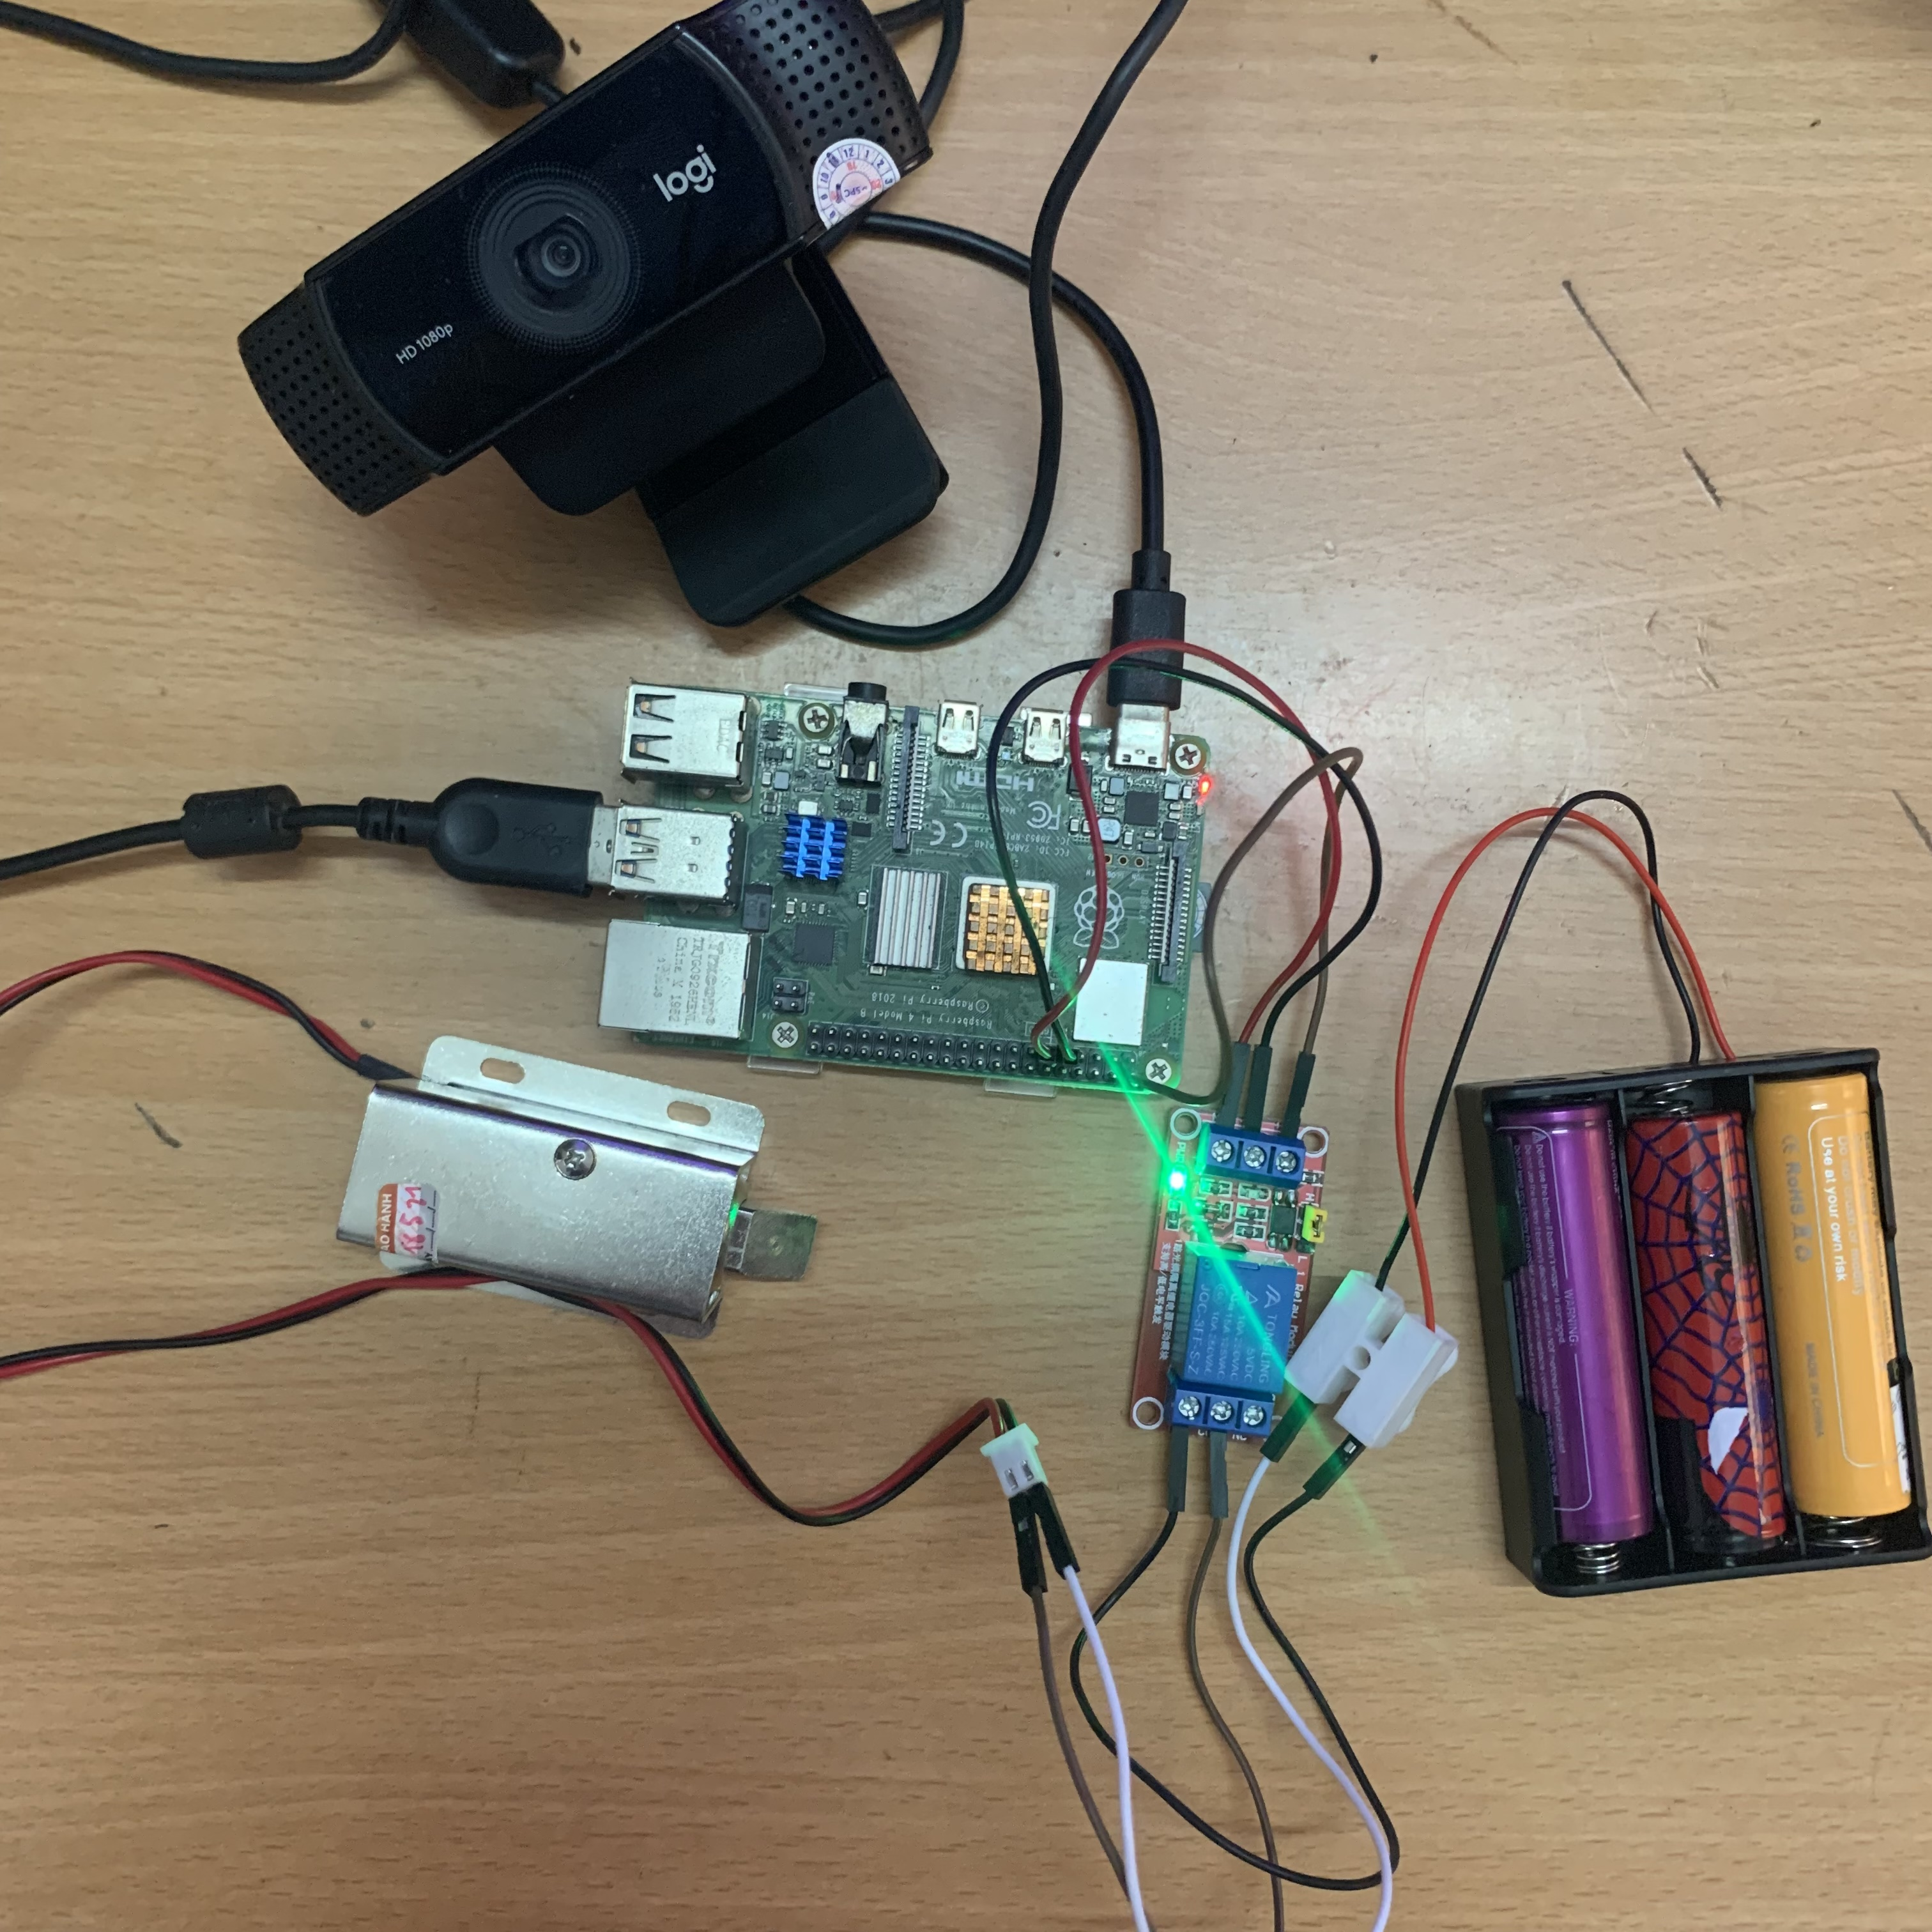
\includegraphics[scale=0.16]{ccuSetup.jpeg}
    \caption{Our door lock setup}
    \label{fig:ccuSetup}
\end{figure}

We have tried to implement the recognition system on the \acrshort{ccu}. Still, since it was relatively computationally and memory intensive, the recognition has the worst performance when running on the \acrshort{ccu}.

